\documentclass[../root]{subfiles}
\graphicspath{{_images/}{../_images/}}

\begin{document}

    \chapter{The Effect of Patient Cost Sharing on Utilization, Health, and Risk Protection}

    \begin{shortsummary}
        \begin{itemize}
            \item \authoryear{Shigeoka2014}
            \item \RQ{How patient cost sharing affects utilization, health, and risk protection, especially among the elderly?}
            \item \answer{RDD using a Japanese national policy that sharply reduces patient cost sharing at age 70.}
            \item \result{Reduced cost sharing at age 70 discontinuously increases health care utilization, especially patients with high medical spending. No any effects on the health measures.}
        \end{itemize}
    \end{shortsummary}

    \section{Introduction}

    \paragraph{Medicare Legislation and Tradeoffs}

    \begin{itemize}
      \item Rising medical expenditures: aging population and coverage expansion.
      \begin{itemize}
        \item More than 1/3 of current health spending is on the elderly; future cost control efforts can be expected to focus on seniors.
        \item The government is to contain health care costs.
      \end{itemize}
      \item Requring patients to pay a larger share of the medicare costs has clear tradeoffs.
      \begin{itemize}
        \item Decreasing the moral hazard
        \item Future severe and costly health events.
      \end{itemize}
      $\Rightarrow$ To help determine the appropriate level of cost sharing, there is an urgent need for knowledge on how patient cost sharing affects utilization, health, and risk protection.
    \end{itemize}

    \paragraph{Literature}

    \begin{itemize}
      \item Credible evidence on the price sensitivity is scarce.
      \begin{itemize}
        \item RAND Health Insurance\footnote{The HIE project was started in 1971 and funded by the Department of Health, Education, and Welfare (now the Department of Health and Human Services). It was a 15-year, multimillion-dollar effort that to this day remains the largest health policy study in U.S. history. The study's conclusions encouraged the restructuring of private insurance and helped increase the stature of managed care. - from RAND} exclude individuals above the age of 62.
        \item Card, Dobkin, and Maestas (2008, 2009): Medicare eligibility at 65 yrs of age discountinuously increases health care utilization and has a modest positive effect on the health of elderly patients above 65 years.
      \end{itemize}
      \item Few studies adress whether the changes are the result of extensive margin(health insurance provision per se) or intensive margin(changes in health insurance generosity).
      \begin{itemize}
        \item Only a few studies in the United States have examined the effect of health insurance on the distribution of out-of-pocket medical expenditures (Feldstein and Gruber 1995; Finkelstein and McKnight 2008; Engelhardt and Gruber 2011; Finkelstein et al. 2012).
      \end{itemize}
    \end{itemize}

    \paragraph{Sharp reduction in cost sharing for patients aged over 70 in Japan}

    \begin{itemize}
      \item Cost sharing for outpatient visits and inpatient admissions is as much as 60–80 percent lower at age 70 than at age 69 in Japan by law.
      \item Advantages
      \begin{enumerate}
        \item No confounding factors at age 70
        \item They can identify the price elasticity of inpatient admissions and outpatient visits separately.
        \item They can examine the effect of cost sharing, rather than health insurance per se, on exposure to out-of-pocket medical expenditure risk.
        \item The unique setting in Japan allows to separate the demand elasticities of patients from responsive behavior by insurers and medical providers.
      \end{enumerate}
    \end{itemize}

    \paragraph{Results}

    \begin{enumerate}
      \item Reduced cost sharing at age 70 discontinuously increases health care utilization.
      \begin{itemize}
        \item The corresponding elasticity is modest, at around −0.2 for both outpatient visits and inpatient admissions.
      \end{itemize}
      \item Lower patient cost sharing improves any of the health measures.
      \item Patients with high medical spending benefit substantially from financial protection against risk due to lower cost sharing.
    \end{enumerate}

    \section{Background}

    \paragraph{Institutional Setting}

    \begin{itemize}
      \item All Japanese citizens are mandatorily covered by health insurance.
      \item Patients have unrestricted choices of medical providers
      \begin{itemize}
        \item Patients have direct access to specialist care without going through a gatekeeper or a referral system.
        \item no limit on the number of visits.
        \item The insurer pays the remaining fraction of expenses until the beneficiary meets the stop-loss, and the insurer pays all expenses above the stop-loss: no deductible
      \end{itemize}
      \item Elderly Health Insurance
      \begin{itemize}
        \item lower cost sharing: The elderly become eligible on the first day of the next month after they turn 70.
        \item also provided to bedridden people between the ages of 65 and 70, but the proportion is not substantial (at most 4.2\%).
      \end{itemize}
      $\Rightarrow$ the estimated price elasticity and health consequences may be interpreted as the lower bound.
    \end{itemize}

    \begin{itemize}
      \item Below 70, Two types of health insurance are provided: After 2003, both were equalized to a common coinsurance rate.
      \begin{itemize}
        \item Employment-based health insurance: covers employees
        \item National Health Insurance: everyone else
      \end{itemize}
      \item After 70: Elderly Health Insurance.
      \begin{itemize}
        \item No incentives for the medical providers to to influence patient demand.
      \end{itemize}
    \end{itemize}

    \begin{figure}[ht]
      \centering
      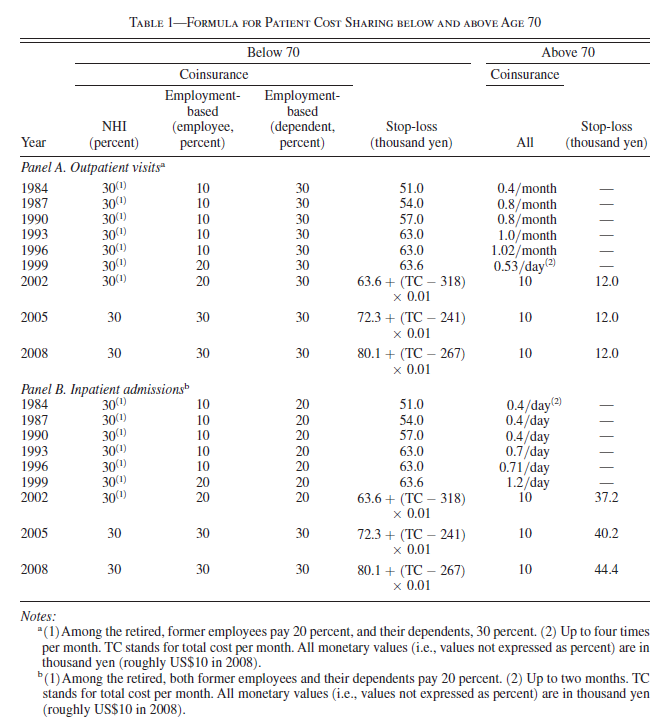
\includegraphics[scale = 1]{0710tanji/T1}
    \end{figure}

    \paragraph{Changes in Patient Cost Sharing at Age 70}

    \begin{itemize}
      \item the stop-loss differs for outpatient visits and inpatient admissions for those over 70.
      \item for any given medical expenditures, the out-of-pocket payment for those above 70 was always smaller than that for those below 70 in 2008.
      \item Using Survey of Medical Care Activities in Public Health Insurance, they computed counterfactual out-of-pocket expenditures by applying the cost sharing rules of Elderly Health Insurance to utilization by an average 69-year-old.
      \begin{itemize}
        \item Summary of the monthly medical expenditures claimed for insurance reimbursement to medical institutions
      \end{itemize}
    \end{itemize}

    \begin{figure}[ht]
      \centering
      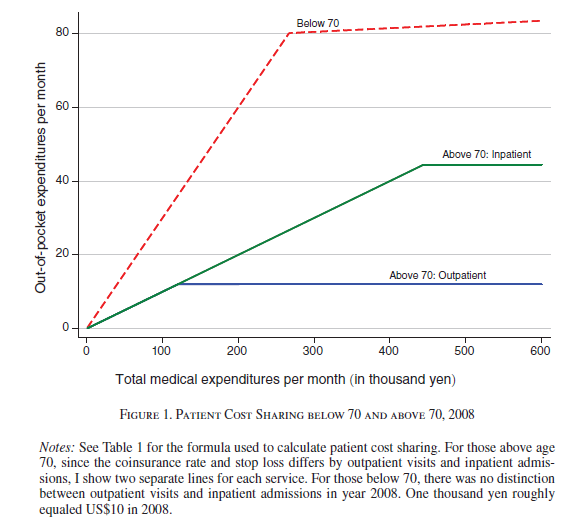
\includegraphics[scale = 1]{0710tanji/F1}
      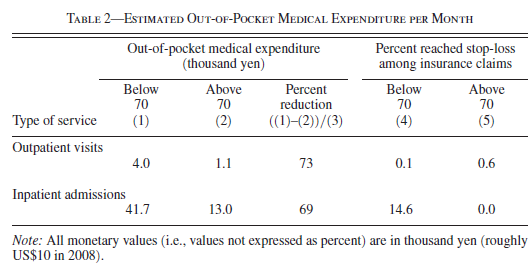
\includegraphics[scale = 1]{0710tanji/T2}
    \end{figure}

    \begin{itemize}
      \item Out-of-pocket medical expenditures for inpatient reduces from 27 percent of a person’s average monthly income (1,822 thousand JPY) to 8.6 percent.
    \end{itemize}

    \paragraph{The Problem of Nonlinearity Imposed by the Stop-Loss}

    \begin{itemize}
      \item Medical expenditure is caused by unpredictable illnesses, but  economically rational individuals who anticipate spending beyond the stop-loss may spend more when the price is low (Keeler and Rolph 1988).
      \item In this paper, the author guesses that the effect of this is small enough for:
      \begin{enumerate}
        \item the probability of reaching the stop-loss is not high even for inpatient admissions
        \item The stop-loss is set monthly in Japan
      \end{enumerate}
      \item the nominal price (41,000 JPY) for those just below age 70 is not so different from the true price (38,000 JPY).
    \end{itemize}

    \section{Data and Identification}

    \paragraph{Data}

    \begin{itemize}
      \item Patient Survey
      \begin{itemize}
        \item A nationally representative repeated cross-sectional survey (every 3 yrs).
        \item Administrative data from hospitals and clinics: individual patient-level data for 9 rounds (1984-2008).
        \item Information on outpatient visits can be recognized.
        \item Individual demographics are limited: gender, place of residence, \ldots, no record of education and income.
      \end{itemize}
      \item Contents
      \begin{itemize}
        \item Utilization:
        \begin{itemize}
          \item the dates of the visits, birth, admission, surgery, and discharge.
        \end{itemize}
        \item Health outcomes
        \begin{itemize}
          \item Mortality: well-defined from the universe of death records between 1984 and 2008.
          \item Morbility: from the Comprehensive Survey of Living Conditions (CSLC) between 1986 and 2007.
          \begin{itemize}
            \item insurance coverage, self-reported physical and mental health, stress levels, \ldots.
          \end{itemize}
        \end{itemize}
      \end{itemize}
    \end{itemize}

    \section{Identification Strategy}

    \begin{enumerate}
      \item Utilization, and Morbidity
      \[
      Y_{iat} = f(a) + \beta \text{Post70} + X'_{imt} \gamma + \epsilon_{iat}
      \]
      \begin{itemize}
        \item $Y_{iat}$: measure of morbidity or out-of-pocket medical expenditure for individual $i$ at age $a$ in survey year $t$.
        \item $f(a)$ is a smooth function of age
        \item $X_{iat}$ individual covariate: set of dummies for gender, marital status, region, birth month, and survey year, fully interected with the $Post$ dummies.
        \item $\text{Post70}$ indicator for aging 70, whose coef. is the parameter of interest.
      \end{itemize}
      \item Mortality, and Patients
      \[
      \log(Y_{at}) = f(a) + \beta \text{Post}70_{at} + \mu_{at}
      \]
      \begin{itemize}
        \item $Y_{at}$: the count of patients or deaths at age $a$ in year $t$.
      \end{itemize}
    \end{enumerate}
    \begin{itemize}
      \item Notations:
      \begin{itemize}
        \item age window: 65-75, while 67-73 in the robustness checks.
        \item the standard errors are clustered at age in months.
        \item the problem of substantial seasonality and heaping in the reported birthdays of patients observed in the Patient Survey.
        \begin{enumerate}
          \item in the first day of each month: Reporting
          \item in the first quarter: Farmers timing of births
        \end{enumerate}
        \begin{itemize}
          \item The author deals this problem by collapsing the data into age in months, and including the birth month fixed effects.
        \end{itemize}
      \end{itemize}
      \item Other complicated problem.
      \begin{itemize}
        \item Patients with unusually long hospital stays: limiting those admitted within three months from discgarge in September.
        \item More deaths in winter
        \item Using death records may attenuate the estimate.
        \item Problem with "age RDD": individuals anticipate the assignment to treatment, which is inevitable

        $\Rightarrow$ the overall age trend does not seem to display any catch-up effects.
        \begin{itemize}
          \item They conducted "donut-hole RDD" (Barreca, Lindo, and Waddell, 2011)
        \end{itemize}
        \item Expected outcomes below and above age 70 are continuous (Hahn, Todd, and Van der Klaauw 2001)
        \begin{itemize}
          \item Employment, marriage, and income are unlikely to confound the impact of cost sharing at the age.
        \end{itemize}
      \end{itemize}
    \end{itemize}

    \section{Utilization Results}

    \paragraph{Outpatient Visits}

    \begin{itemize}
      \item Output visits junp at age 70, by 10.3\% (Panel A)
      \begin{itemize}
        \item The implied elasticity is -.18 = $\frac{.103}{\log(1.1) - \log(4.0)}$.
        \item The increase appears to be permanent without reverse to the previous level.
        \item Dividing sample before and after 2002 yields relatively similar results (elesticity of -.19 and -.15, respectively.)
      \end{itemize}
      \item The duration from the last visit and drops sharply by roughly one day at age 70.
      \item Source of the increasing utilization.
      \begin{enumerate}
        \item Moral hazard
        \item Increases in beneficial care
      \end{enumerate}
      (Table 3)
      \begin{itemize}
        \item First visits increase at the age 70, as well as repeated visits.
        \item The increase (17.9\%) occur among those vists within one day from the last visit.
        \item By type of diseases.
        \begin{itemize}
          \item Diagnosis listed as ACSCs; modest jump at 70.
        \end{itemize}
      \end{itemize}
    \end{itemize}

    \begin{figure}[ht]
      \centering
      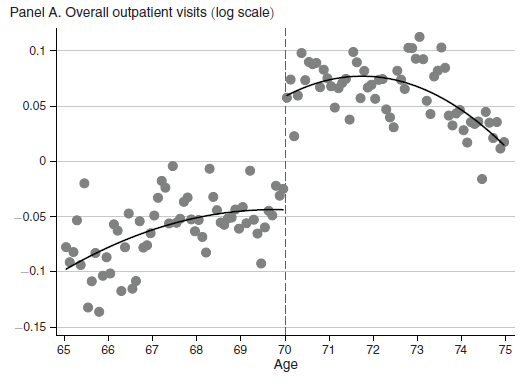
\includegraphics[scale = .8]{0710tanji/F2a}
      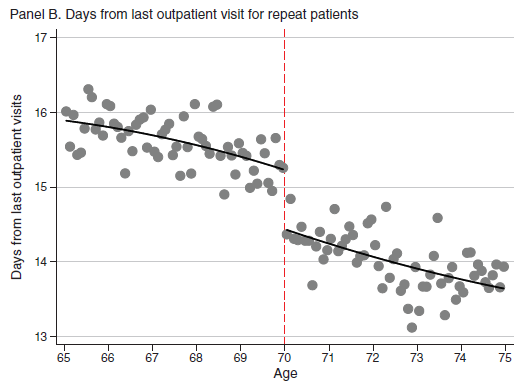
\includegraphics[scale = .8]{0710tanji/F2b}
    \end{figure}

    \begin{figure}[ht]
      \centering
      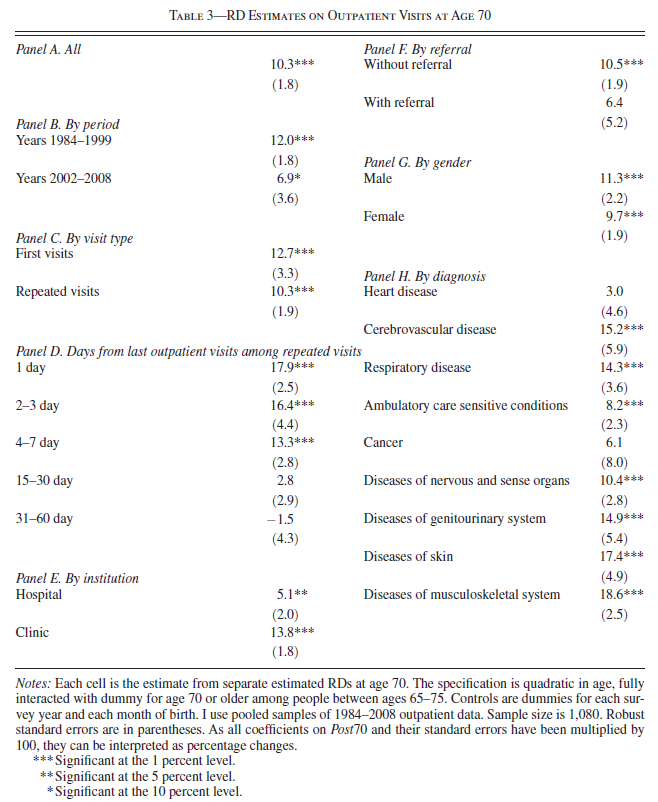
\includegraphics[scale = 1]{0710tanji/T3}
    \end{figure}

    \paragraph{Inpatient Admisssions}

    \begin{itemize}
      \item Impatient admissions jumps at age 70, by 8.2\% (Panel A)
      \begin{itemize}
        \item The implied elasticity is -.16 = $\frac{.082}{\log(13.0) - \log(41.7)}$. (-0.14 by donut-hole RD)
        \item Using different window yields similar results.
      \end{itemize}
      \item Another bias source: forward-looking behavior the timing of admission within a month

      $\Rightarrow$ Deviding the sample patients admitted in the 1st/2nd half of the month yields the same result.
      \item Possible Mechanisms
      \begin{itemize}
        \item Some people who are close to 70 years of age delay surgery until they become eligible for Elderly Health Insurance.
        \item Using the fraction of weekend admissions as a severity measure $\Rightarrow$ clear negative relationship.
        \item Type of diagnosis: consistent with ard, Dobkin, and Maestas (2008):
        \begin{itemize}
          \item Diagnoses that are treated with expensive but elective procedures are quite price sensitive
        \end{itemize}
      \end{itemize}
      \item Few incentives for medicare providers: Fang and Rizzo (2009) pointed out that recent organizational changes might have fostered patient-initiated requests for specific treatments.
    \end{itemize}

    \begin{figure}[ht]
      \centering
      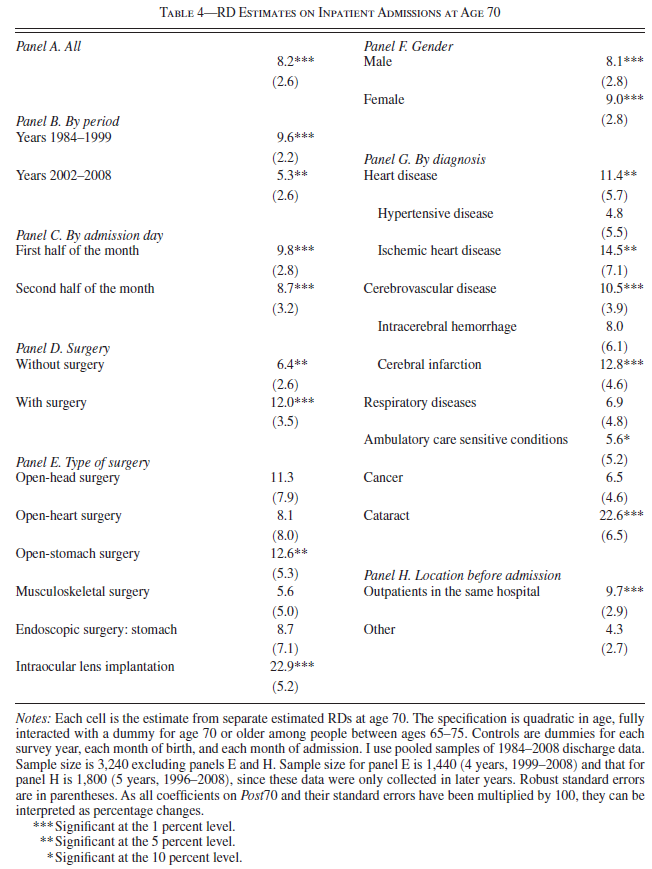
\includegraphics[scale = .8]{0710tanji/T4}
    \end{figure}

    \begin{figure}[ht]
      \centering
      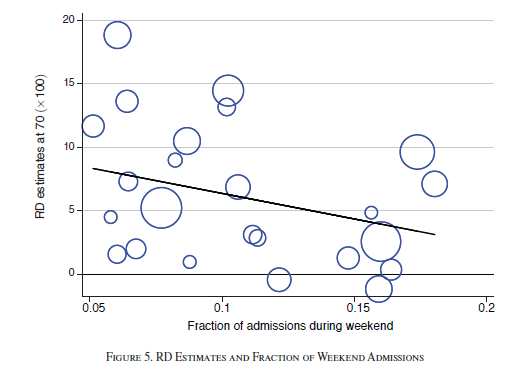
\includegraphics[scale = 1]{0710tanji/F5}
    \end{figure}

    \section{Benefits}

    \paragraph{Health Outcomes}

    \begin{itemize}
      \item The effect of cost sharing is ambiguous: cheaper access to health care vs. delayed life-saving treatment.
      \item The log of overall deaths: no statistically significant effect (-.2 percent).
      \begin{itemize}
        \item Using cause-specific deaths yields the same result.
      \end{itemize}
      \item The results are expected:
      \begin{itemize}
        \item The difficulty to detect the effect on health in RDD (Grossman 1972)
        \item Self-reported physical and mental health yieldds the same.
      \end{itemize}
      \item While there are some possible underestimation, the author does not detect a substantial health effects.
    \end{itemize}

    \paragraph{Risk Reduction}: A lower risk of unexpected out-of-pocket medical spending.

    \begin{itemize}
      \item For risk-averse individuals, the largest welfare gains from lower cost sgaring come from rducing catastrophic negative shocks to consumption (McKnight, 2008; Zackhauser, 1970).
      \item Using CSLC self-reported expenditure, based on 66,112 individuals aged between 65 and 75 years\footnote{The expenditure includes one that is not covered by health insurance}.
      \begin{itemize}
        \item The average annual out-of-pocket spending aged 65-69 is 142,000 JPY, while median 48,000JPY.
        \item The top 5\% of spenders (account for almost 40\% of total spending) receove the largest decline.
      \end{itemize}
      \item Patients at the right tail of the distribution are substantially benefited from lower cost sharing from the reduction in age 70.
    \end{itemize}

    \begin{figure}[ht]
      \centering
      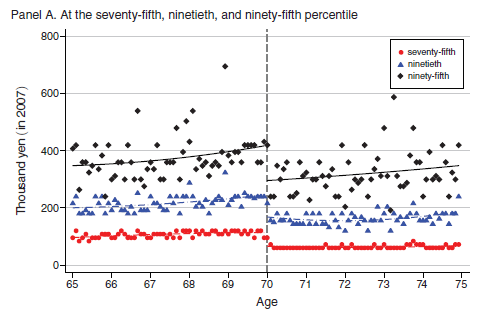
\includegraphics[scale = 1]{0710tanji/F7a}
    \end{figure}

    \section{Discussion}

    \paragraph{Implications of Price Elesticities}

    \begin{itemize}
      \item Patient cost charing affects on two services: inpatient admissions and outpatient visits.
      $\Rightarrow$ How to distinguish the cross-price effects?
      \begin{itemize}
        \item Results for some diagnosis where cross-price effects should be nearly zero can be utilized.
        \begin{itemize}
          \item hypertensive disease: the diagnosis group with highest fraction of outpatient care yields an RD estimate of 8.2\% (10.3\% overall)
          \item benign neoplasm: 11.7\% (8.2\% overall)
        \end{itemize}
      \end{itemize}
    \end{itemize}

    \paragraph{Comparison to Prior Literature}

    \begin{itemize}
      \item It is not clear a priori whether the elderly are expected to have larger or smaller price eleciticies of demand for health care than the non-elderly.
      \item Estimate in this paper is within the range of similar estimates in prior literature.
      \begin{itemize}
        \item Chandra, Gruber, and McKnight (2020)
      \end{itemize}
      \item Many institutional differences between Japan and the United States.
      \begin{itemize}
        \item the ratio of medical expenditure to GDP
        \item Japan’s universal coverage without the need to go through a gatekeeper or a referral system
        \item Physician consultations per-capita per year are 13.2 in Japan, which are more than three times as large as those in the United States (3.9).
        \item The life expectancy at birth was 82.7 in Japan and 78.1 in the United States (OECD 2012).
      \end{itemize}
    \end{itemize}

    \paragraph{Cost-Benefit Analysis}

    \begin{itemize}
      \item The welfare gain of risk protection from lower patient cost sharing is comparable to the total social cost.
      \item One limitation of this welfare analysis is that it does not incorporate welfare gains from health improvements.
    \end{itemize}

    \section{Concluding Remarks}

    \begin{itemize}
      \item This paper overcomes the difficulty to separate the effect on patients from the responsive behavior by medical providers and insurers.
      \item One limitation
      \begin{itemize}
        \item Long-run health benefit into account in this framework may yield additional implication.
      \end{itemize}
    \end{itemize}


    \biblio

\end{document}
